\section{System Architecture}
\label{sec:system_architecture}
The architecture is the most crucial part of the system that designates the relationships between each components. How components are connected, their interaction, and the behaviour of the system with the reasoning for the requirements and problems discussed. How system make decision, handle situation, manage all parts of it are all explained in this section.

This section explains computation steps, more detailed data communication strategy, software architecture, and user interface design specifications as well as critical implementation details. Following two sections, section \ref{sec:server_client} and section \ref{sec:user_interface} explains these aspects in detail.

\subsection{Server - Client Model}
\label{sec:server_client}
\subsubsection{Reasons and Requirements}
Image processing and real time decision making are computationally expensive tasks which come with computational burden. There are also basic requirements which are important for the regular and stable operation of the system. In order to satisfy those requirements and reduce cost in addition to more flexible operation, server - client model best fits for the product. There are many reasons regarding the model structure from the point of customer and the company.

Customer needs and demands are changing continuously, even faster than it had been in past, such that customers are now looking for augmented product features, after-sale services, customer support, maintenance, repair, etc. Moreover, in the scale of thousands of product sales, it is apparent that massive customer support due to failures or malfunctions, questions and suggestions related to the product will require a big budget in the company. In addition, customer desire for monitoring the system and cat statistics are going to be satisfied through a server at present. All of these requirements and specifications make it reasonable to use server - client model.

Server - client model provides very powerful ways to satisfy augmented product requirements. After sale services can be ensured over network; any errors, warnings, malfunctions can be solved in real time, even before customer recognizes it. Digital world also enables customer to find their wants and answers for their products. Sensor data, images, statistics, problems are gathered and manipulated on servers make it possible to satisfy customer needs much faster and quicker. Customized experience for the users can easily be done, end even after the sale they can be reached and powerful customer experience can be achieved. This model also allows the Felerest group to remotely control, update, and collect data in a single way. New updates, modifications, features can be added easily and cheaper. Therefore, server - client model forms the project core and used in practice. Some of requirements for this sub-system is given in the itemized structure shown.

\begin{itemize}
    \item Real time decision making capability
    \item Transfer data without any trouble and loss
    \item React to environmental changes accordingly
    \item Detect dangerous situations and take cautions
    \item Collect sensor, camera data for later analysis
    \item Process data efficiently
    \item Use reasonable amounts of bandwidth
    \item Manage database, dump unnecessary information
\end{itemize}

\subsubsection{Software Design}
The software combines all the parts and creates a backbone for the operation. Modular architecture with agile development is used throughout the project. python is used because of it's flexibility and it's rich library support as well as a big community. New libraries always can be found and errors are easily be solved with the help of community. Moreover, it's abstraction design make it the proper language for the backbone. Note that many programming languages are used in practice, C, bash scripting, JS, PHP; however python is the base language that runs the system.

The system can be explained best in the overall system diagram in \ref{fig:overall_system_diagram}. Controller is the mainframe that governs the whole system. Single server - multiple clients model is used so that the requirements can be satisfied effectively. Each product represents a client, and all of their data is collected in a server for processing, storage, and management. This allows the system to have greater computational capacity and storage size.

% TODO - alttakilerin benzerleri overall icinde de olacak
\paragraph{Client}
Client is the product itself as mentioned earlier. Peripheral communication and environmental controls are the jobs of this module as explained in overall design. Client have three sub-modules which are GPIODriver, CameraDriver, and Client object which separates into Command Client and Video Client. GPIODriver is the controller for the input/output whereas CameraDriver is an abstraction class over Raspberry Pi camera for an easier and clear implementation. Client objects are for video and command transfer which is explained in the next paragraph, namely "Data Communication". As mentioned earlier, all of these abstractions are helpful for connecting various components.


\paragraph{Data Communication}
Data communication consists of every data, no matter type of it. The design suggests two parallel communication channels over TCP/IP protocol which is the only protocol used in data communication for reliability and cheaper implementation cost. The transfers use two separate ports over TCP/IP protocol which can be configured for customization but using 10002 and 10003 by default. These ports do not belong to any known service, therefore port filtering or any other service running in parallel will not be affected.

Everything comes with a cost, data communication does also. Opening data to the internet makes it vulnerable for possible attacks and customer privacy becomes an important issue. Some strategies are developed so as to cope with all of these challenges. Turkey puts some regulations on data transactions one of which is the "Protection of Personal Data" (6698 Sayılı Kişisel Verilerin Korunması Kanunu, Madde 3). This code states that without approval of the customer, it is not possible to store these data on abroad servers which is why servers will be located in Turkey and data privacy on an international scale will be solved. Moreover, encryption for both data, frame or video, and command are encrypted through 4096-bit RSA keys which are considered to be secure \cite{cite:RSA}. Implementation is based on SSH tunnelling, using OpenSSH.

\paragraph{Server}
Server resembles to the client. It uses sub-modules to create the server module. Controller, Classifier, Identifier, and User Interface are the parts creating the server side. Encapsulation of the software is done with python3 in which the most of the code is written. On the other hand, modules requiring high speed, computation burden are written in C, or they are compiled from C libraries such as SIFT, neural networks. Server is responsible for decision making, data storage, statistics, and human interaction for further product updates.

Data, as mentioned earlier, is another problem. It's security, transmission, storage creates problems for even very large servers. Solving these problems requires more strict specifications. For the final prototype, Linux file system with "pickle" objects are used for databases. However, this does not mean the final product is going to have simple file systems. Encrypted SQL databases, distributed storage techniques are future work after the prototype which involves data science and security engineer optimizations. For the prototype, these are omitted and it is assumed the server disk is completely secure, or it is run under a human supervision.


\subsection{Tests and Results, Future Test Plans}
Tests are measured with software tools nethods, top, iotop, and system monitor. The system results are given for the personal computer located in Computer Engineering Department Laboratories in METU. Taken 10 data points are averaged to get these results.

\begin{verbatim}
    121 KB/s network usage on average
    1.7 lag in data transmission
    0.0625 errors / min
    Memory (server) : 624 M
    Memory (client)  : 1.99 M
    CPU (server) : 13.3 %  (i7-4770S)
    CPU (client)  : 2.2 %  (ARM1176(+)
\end{verbatim}



\subsection{User Interface}
\label{sec:user_interface}

This module deals with the delivery of information regarding the device and its cats to the owner (user) of the device via the Internet. Following are the required features:

\begin{itemize}
    \item Device's food supply level
    \item Device's battery level during charging
    \item Device's battery level during operation
    \item Device's feeding log
    \item Cats' profiles
\end{itemize}

An explanation and reasoning of the requirements is due:

\textbf{Food Supply: } Food supply level information helps the user decide when to refill the food tank. How the information is obtained is explained in detail in Section \ref{sec:electrical_design}.

\textbf{Battery Level: } This is essential for any rechargeable product. Detailed explanation will follow in Section \ref{sec:electrical_design}.

\textbf{Feeding log: } Each device has a feeding log of all cats that have been fed from it since its setup.

\textbf{Cat profiles: } These profiles are initially handled by the Identification module. (see 4.\ref{sec:identification}. Each profile includes a name, an image and an individual feeding log. Furthermore, the name attribute is initially 'name' and can be edited later on by the user of the device. Nonetheless, the user cannot edit his/her cats' images: the images are provided by the device's camera. Feeding log is also not to be edited.

% justify istiyor iste, biliyordum falan diyebilirsin tecrubem vardi, cpu time dusuk falan, ek sunucu ihtiyaci yok, python ile iletisim kuruyor

For the interface, a Python web framework called Flask is used. There were a few reasons behind this choice:

\begin{itemize}
    \item Our user interface and web designer, Furkan, had more experience in Flask than in other frameworks.
    \item Since Flask uses Python in the background, CPU time is less than other platforms such as Nodejs.
    \item There is no need for an additional server, since a command as simple as `flask run' can let us run our website on our computers.
    \item Because the communicated modules are mostly developed in Python, the communication is seamless.
\end{itemize}

The user interface, prototype of which is currently hosted on \\ \href{https://felerest.pythonanywhere.com/}{felerest.pythonanywhere.com}, consists of 3 main pages: devices page, cats page, settings page, all of which can be accessed only with the user's password.

\clearpage

\begin{figure}[ht] 
     \centering
     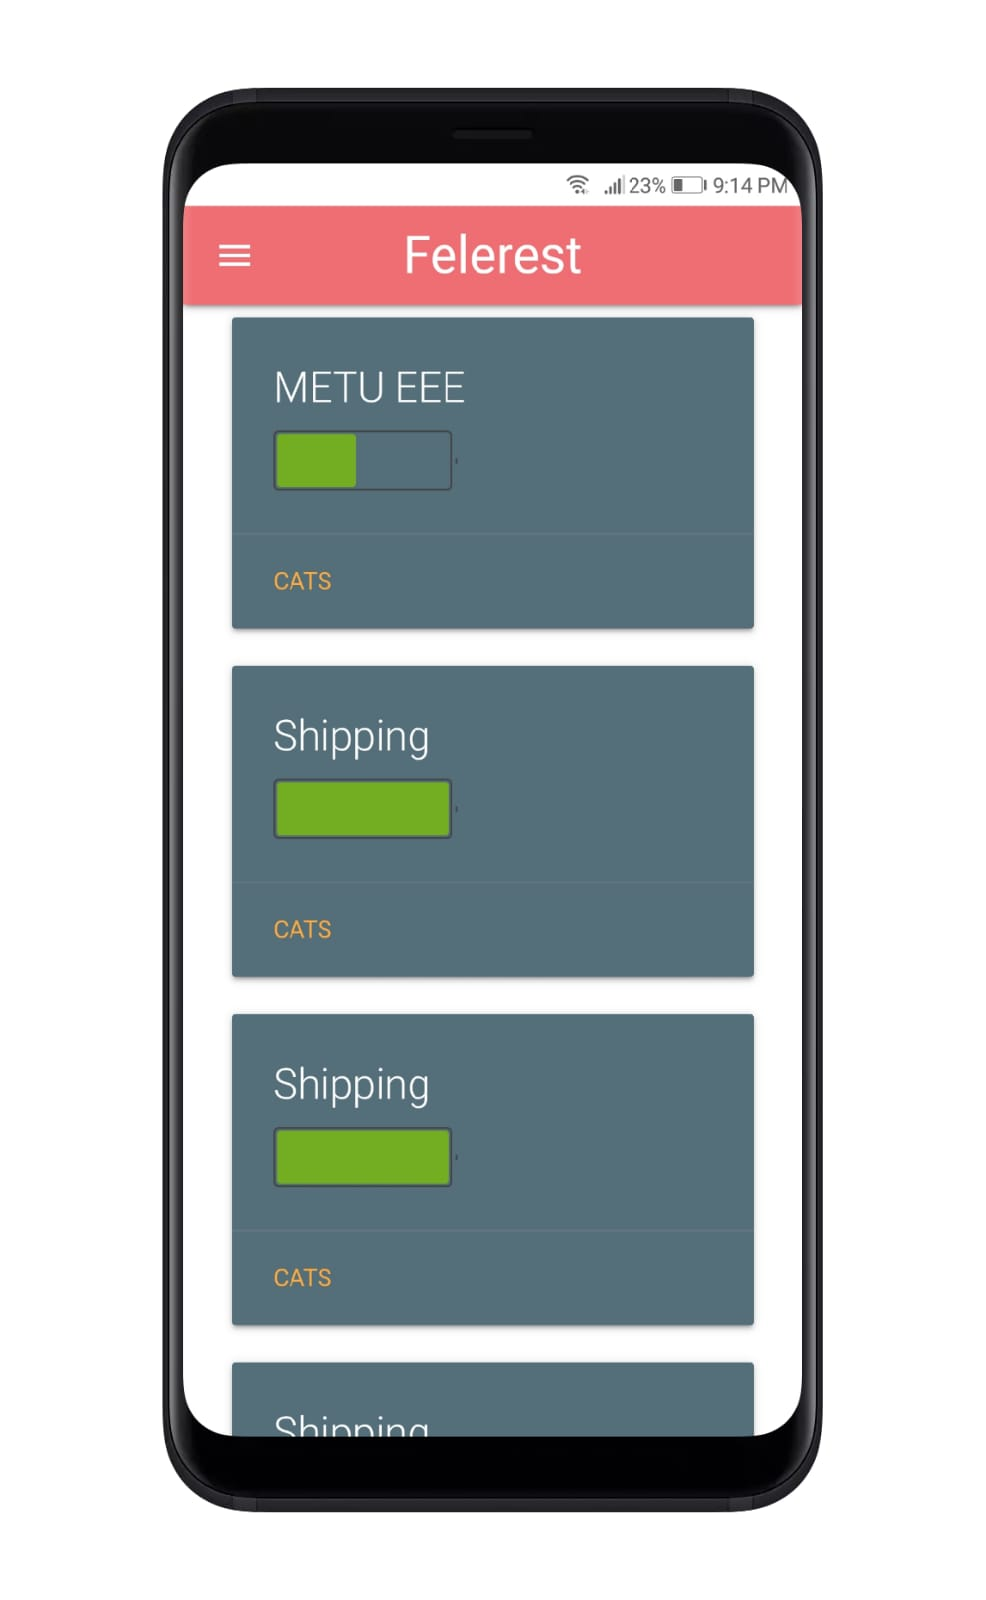
\includegraphics[width=.55\linewidth]{content/030_system_architecture/img/user_interface/devices.jpeg}
     \caption{User Devices Page}
     \label{fig:ui-devices}
\end{figure}

The devices page (Figure \ref{fig:ui-devices}) displays all devices that the user owns as cards in a grid. Each card shows that particular device's location, battery level, and food supply level. The food supply level indicator will be added eventually. There is also a link at the bottom of each card that takes the user to that device's cats page. There will also be another link that displays the entire feeding log of the device.

Cards in the figure labeled Shipping are just dummy devices to test the behavior of the grid with multiple cards.


\begin{figure}[ht]

\begin{subfigure}{0.5\textwidth}
    \centering
    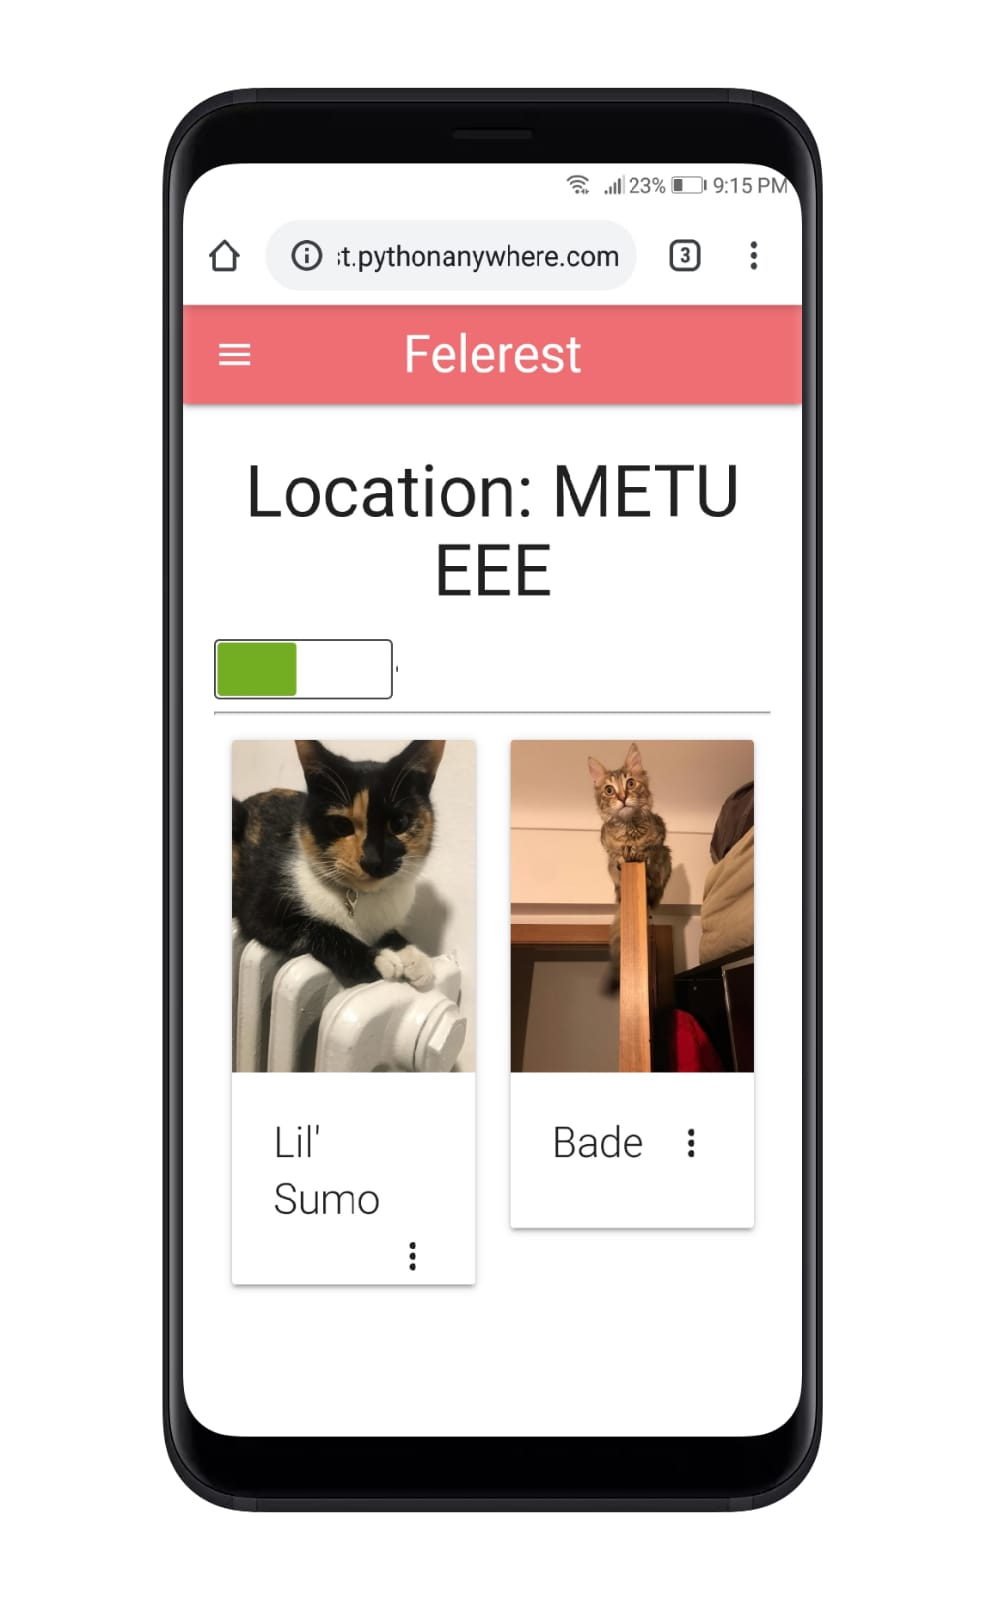
\includegraphics[width=\linewidth]{content/030_system_architecture/img/user_interface/cats.jpeg}
    \caption{Device Cats Non-revealed}
    \label{fig:ui-cats}
\end{subfigure}
\begin{subfigure}{0.5\textwidth}
    \centering
    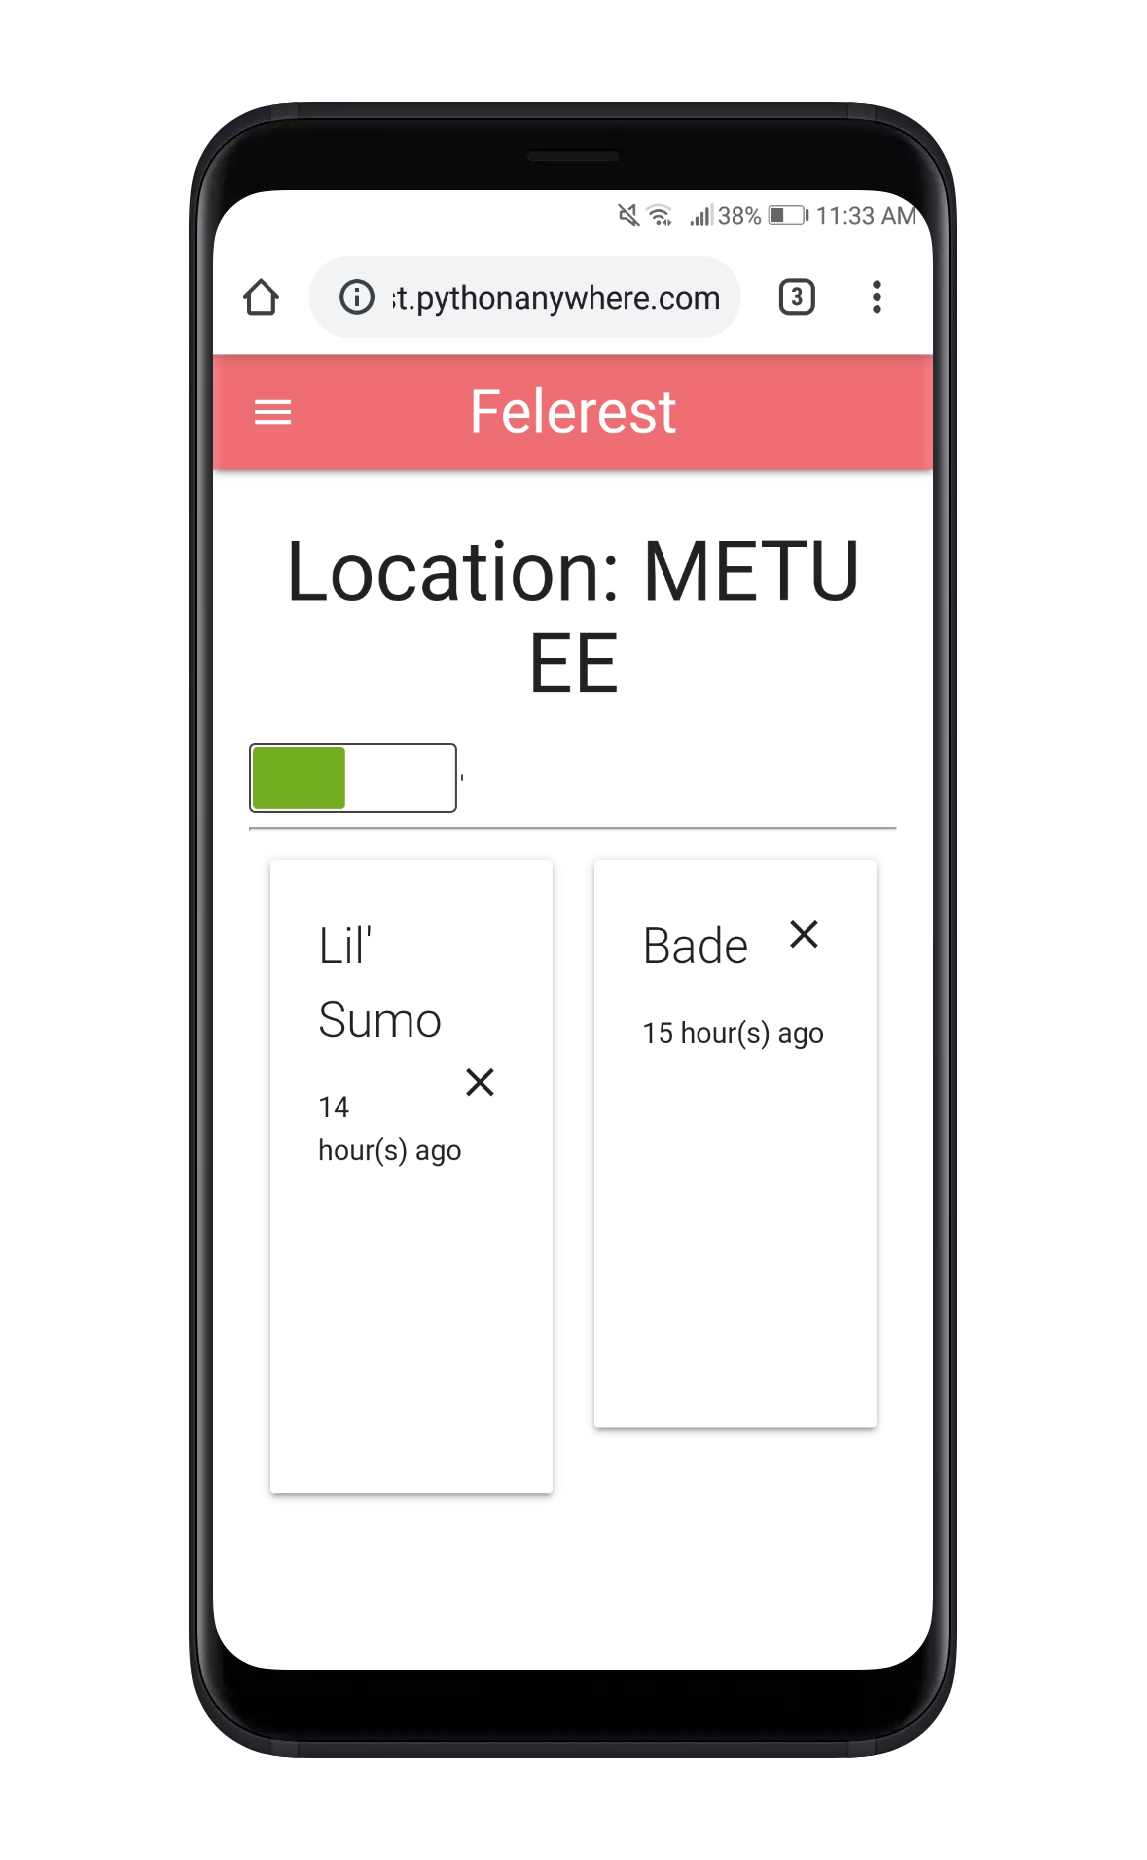
\includegraphics[width=\linewidth]{content/030_system_architecture/img/user_interface/cats_revealed.png}
    \caption{Device Cats Revealed}
    \label{fig:ui-cats-revealed}
\end{subfigure}
\caption{Device Cats Page}
    \label{fig:ui-cats-combined}
\end{figure}

The cats page (Figure \ref{fig:ui-cats-combined}) displays all cats that belongs to a device. On the page, the location, battery level, and food supply level of the device is displayed again for convenience of the user. Moreover, each cat has its own card that displays a name and an image. When the user clicks on a cat's card, the last feeding time of the cat is revealed, along with a link to the cat's feeding log. Currently, only the last feeding time is implemented.

\begin{figure}[h!] 
     \centering
     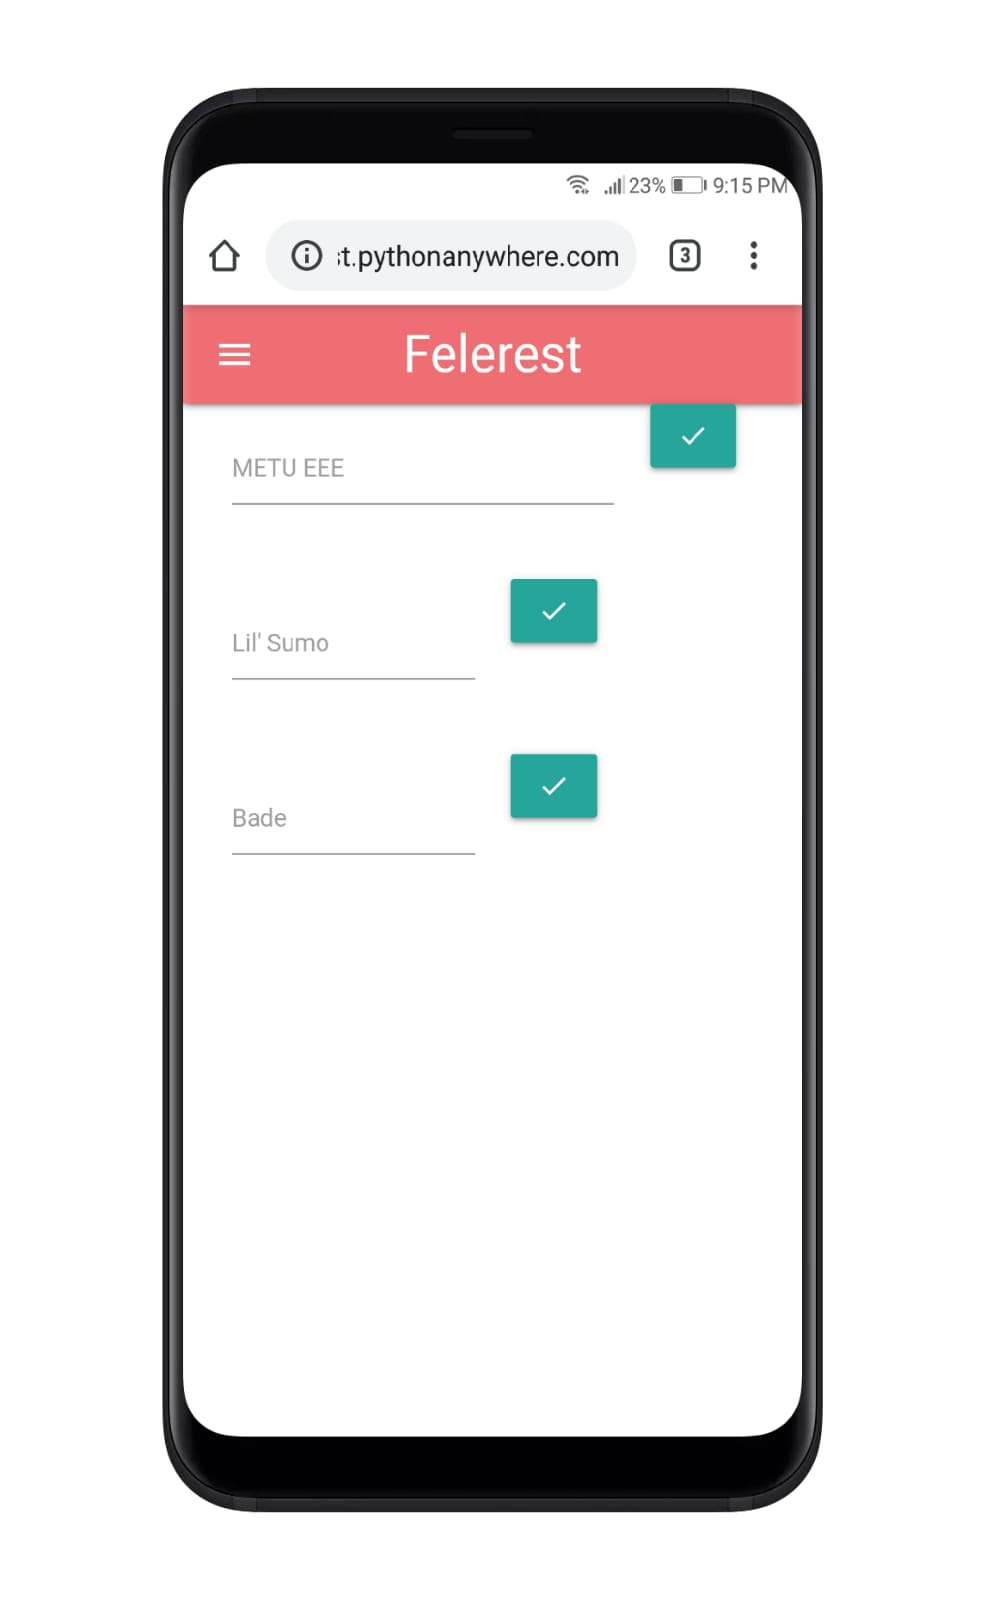
\includegraphics[width=.55\linewidth]{content/030_system_architecture/img/user_interface/settings.jpeg}
     \caption{User Account (Settings) Page}
     \label{fig:ui-settings}
\end{figure}

The last essential page, the settings page, can be seen in Figure \ref{fig:ui-settings}. Here the user can change the locations of devices and names of cats that are affiliated with him/her. The changes that are done here are implemented instantly. Locations/names `METU EEE', `Lil' Sumo', and `Bade' have all been given as inputs to this page.

\clearpage


% \subsection{Decision Making}
% \label{sec:decision_making}
% \input{content/030_system_architecture/decision_making.tex}